\subsection{Limitations}
\label{sec:current-limitations}

% Short intro
Different sources of errors and potential improvements can be identified for improving the accuracy of the models.
This section discusses those errors and how improvements can be implemented.

\subsubsection{Impact of fixed failure threshold}
\label{sec:fixed-failure-threshold}

% Explain why the fixed failure criteria is wrong
The simulation presented earlier (Fig. \ref{fig:reference_simu}) clearly showed that the fixed threshold is a major source of modeling error.
The problem was particularly clear for the amplitude of signal V\textsubscript{1p0}.
Indeed, a fixed failure criteria leads to an oversimplification of the output waveform model, as illustrated by Fig. \ref{fig:impact-single-failure-criteria}.
The green waveforms show the case where the failure is not recorded, and the curve model is simply flat and constant (V\textsubscript{OUT} model).
The red waveforms show the case where a failure is well recorded, but the amplitude of the original signal goes way beyond the failure criteria.
In this case, the curve model amplitude (V\textsubscript{OUT} model) is not large enough and does not match V\textsubscript{OUT}.

\begin{figure}[!h]
  \centering
  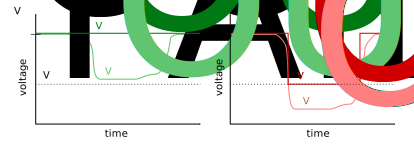
\includegraphics{src/4/figures/bad_output_modelling.pdf}
  \caption{Lack of accuracy caused by the use of a single failure criteria to model the output}
  \label{fig:impact-single-failure-criteria}
\end{figure}

%
Originally, the fixed failure criteria was used for historical reasons.
It came from characterization of hard-failure robustness performed with Wunsch and Bell method \cite{wunsch-bell}.
The methodology presented in this document started directly from this approach, and a first prototype was implemented using this same fixed failure criteria.
In regard of the results presented earlier, the applicability of this fixed threshold for modeling soft-failure of analog block functions has been questioned.
The analysis in this section demonstrated that \textbf{a fixed failure threshold is not suitable in the modelization of analog blocks}.
This major observation is confirmed in the next section that discusses the impact of the fixed characterization load.

\subsubsection{Impact of characterization output load}

% First source of error - load impedance
Previously, all characterization curves were extracted with a fixed output load of 1M\textOmega{}.
This value was selected because it is rather high-impedance and does not prevent proper circuit operation.
It also draws a non-negligible amount of current and reproduces the circuit load of the complete schematic.
It is possible that this fixed high-impedance load is a factor of error for the model chain.

% Compare 1Mohm with real case where blocks are connected together
In practice, each block sees a load impedance on its output much different than 1 M\textOmega{}.
For instance, the output of the pre-regulator is used as a supply by other blocks.
It can deliver a maximum of 20 mA of current while maintaining 8V, corresponding to a minimum output load this block can sustain is 400 \textOmega{}.
The bandgap, on the other hand, provides a reference voltage at 1V but does not deliver a lot of DC current.
More than 1uA is enough to make the output fall of a hundred millivolts.
In this case, the bandgap must see an output impedance of at least 1 M\textOmega{}.

% What is done next
To evaluate this impact, the pre-regulator is characterized again by with 4 different load values ranging from 500 \textOmega{} to 1 M\textOmega{}.
Results are summarized in table \ref{tab:impact-load-on-cz}.
The three first column represent the input parameters, and the last column shows for how long the output was disturbed.
The duration is measured using the failure criteria of the pre-regulator (V\textsubscript{clamp9} < 0V).
It is the time during which the failure criteria was violated.

% Table observation
For the smallest 10V stress amplitude, the failure time is largely impacted by the output load.
The worst case is for the -10V 1\textmugreek{}s pulse (Table \ref{tab:impact-load-on-cz}).
The output goes below 0V for 1330 ns with 500\textOmega{} on the output, but with 1M\textOmega{}, no failure is observed.
However, it is interesting to notice that for larger pulse amplitudes (below -30V), the output load has a limited impact on the failure duration.

% Analyse the table
Those observations tend to indicate that once the output is at fault, having 500\textOmega{} or 1M\textOmega{} connected to it doesn't change the period during which it remains at fault.
This is a major observation, because it shows that the output load value is not a key parameter during the characterization, and that the 1 M\textOmega{} value is sufficient for this study case.

\begin{table}[!p]
\centering
\begin{tabular}{llll}
\toprule
load (\textOmega) & amplitude (V) & length (ns) & output disturbed (ns)   \\ \midrule
500               & -10        & 10         & 10n    \\
5k                &            &            & 1n    \\
50k               &            &            & None    \\
1M                &            &            & None    \\
\rowcolor[gray]{.95}
500               &            & 100        & 100n    \\ \rowcolor[gray]{.95}
5k                &            &            & 1n    \\ \rowcolor[gray]{.95}
50k               &            &            & None    \\ \rowcolor[gray]{.95}
1M                &            &            & None    \\

500               &            & 1000       & 1330n    \\
5k                &            &            & 1289n    \\
50k               &            &            & None    \\
1M                &            &            & None     \\
\rowcolor[gray]{.95}
500               & -30        & 10         & 20n    \\ \rowcolor[gray]{.95}
5k                &            &            & 10n    \\ \rowcolor[gray]{.95}
50k               &            &            & 10n    \\ \rowcolor[gray]{.95}
1M                &            &            & 10n    \\

500               &            & 100        &  506n   \\
5k                &            &            &  580n   \\
50k               &            &            &  594n   \\
1M                &            &            &  594n   \\
\rowcolor[gray]{.95}
500               &            & 1000       & 2087    \\ \rowcolor[gray]{.95}
5k                &            &            & 2194    \\ \rowcolor[gray]{.95}
50k               &            &            & 2206    \\ \rowcolor[gray]{.95}
1M                &            &            & 2206    \\

500               & -45        & 10         & 46n    \\
5k                &            &            & 10n    \\
50k               &            &            & 10n    \\
1M                &            &            & 10n    \\
\rowcolor[gray]{.95}
500               &            & 100        & 657n    \\ \rowcolor[gray]{.95}
5k                &            &            & 715n    \\ \rowcolor[gray]{.95}
50k               &            &            & 717n    \\ \rowcolor[gray]{.95}
1M                &            &            & 727n    \\

500               &            & 1000       & 2668n    \\
5k                &            &            & 2764n   \\
50k               &            &            & 2800n    \\
1M                &            &            & 2800n    \\

\bottomrule
\end{tabular}
\caption{Impact of the output load on characterization results}
\label{tab:impact-load-on-cz}
\end{table}

% Visual explanation of why the impact of the load at small amplitude
Fig. \ref{fig:impact-time-domain-load} provides a visual representation of this observation, which is helpful for understanding this result.
When the output is disturbed and its amplitude is near the failure criteria, the load value has a strong impact on the width of the failure.
This is represented by the green curve in Fig. \ref{fig:impact-time-domain-load}.
A large load value such as 1 M\textOmega{} decreases the amplitude a little bit, causing the output to be above the failure criteria.
With 1 M\textOmega{}, no failure is recorded.
With a small load value (500 \textOmega{}) the output amplitude is increased a little bit (it becomes more negative).
This time, it is below the failure criteria and a failure is recorded.
This explains how the load has a large impact of the failure width for small stress amplitudes.

\begin{figure}[!h]
  \centering
  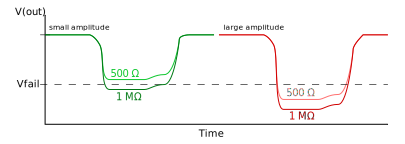
\includegraphics{src/4/figures/zout_impact_time_domain.pdf}
  \caption{Represented impact of output load impedance on the output waveform during a disturbance with a small amplitude (green) and a large amplitude (red)}
  \label{fig:impact-time-domain-load}
\end{figure}

% Explanation at large amplitude
For large stress amplitude (red curve of Fig. \ref{fig:impact-time-domain-load}), the amplitude variation caused by a 500 \textOmega{} load versus 1 M\textOmega{} is not sufficient to change the outcome.
In both cases, a failure will be recorded.

% Conclusion, the main impact is not the characterization load, but the single failure criteria
In conclusion, the load value used during characterization does not seem to be the main source of error.
Once again, it is proven that a fixed failure criteria is a major issue and limiting factor.
It is responsible for the large variations observed in Table \ref{tab:impact-load-on-cz} at small amplitudes.
This result correlates with the observation made earlier in section \ref{sec:fixed-failure-threshold}.

\subsubsection{Preliminary conclusion}

% Conclusion - fixed threshold sucks
Two different sources of errors were analyzed in this section.
It was established that the fixed failure threshold is unsuitable for characterizing and modeling analog block functions.
It should also be noted that defining this fixed threshold is an issue in itself, because very often a purely arbitrary value has to be chosen.
In some rare cases, the specification could be used to set this criteria, but it remained mostly an arbitrary level.
For digital cells, a fixed criteria is correct because above a certain input level disturbance an output can be switched and the failure is clear.
However for the analog domain this rationale does not apply, because for most analog functions there is no clear failure.
Most nets will have degraded values until extreme levels are reached where biasing might completely fail.
Sometimes, the product is destroyed before reaching those extreme levels.
In any case, the fixed threshold hides a lot of information about the degradation.

% Secondary issue
It was also suspected that the output load used during characterization might impact the results too much.
In practice, it was proven in the case of the regulator that this is not exactly true.
Changing the load can induce a variation, but seemingly more limited than the impact of the fixed failure criteria.

% Next
In the next section, a modification is brought to the characterization and modeling method.
The fixed threshold is removed and replaced by a more flexible and powerful solution.
